
\chapter{Background and Theory}
\label{cha:bib}
\section{Background Overview}
\qquad Decision-makers in a number of areas, such as transport, urban planning and education, will benefit immensely from the large amount of data available from various data sources, such as roadside traffic sensors, mobile phone tracking \cite{lopes2010traffic} and social media. But the data obtained through these approaches are vulnerable to data quality (DQ) issues, such as imprecision, incompleteness and heterogeneity\cite{hutchins2008probabilistic} \cite{jagadish2014big}. In recent years, data management techniques for data profiling, cleaning and integration have been uesd to improve the quality of raw data, during preparation for futher analysis or for machine learning. As more and more unstructured data (e.g., text written in natural language) becomes a component to be integrated with other types of data before analysis can be performed, challenges associated with Natural Language Processing (NLP) need to be addressed in this scenario. 

Because this project is to use NLP technology to generate data from natural language data source and implement data integration with traffic sensor data, this chapter will investigate the related background, techniques, and methods about data collection, text classification, language model, neural network, named entity recognition, information extraction, data integration.Furthermore, a number of important and representative studies will be reviewed. 
\section{Web Scraping}
\qquad In order to obtain reliable natural language information, we need to grab traffic-related news information from the news website. Therefore, how to automatically obtain valuable information on the page, especially natural language information, is the first problem to be solved in this project. If a website provides a specific API for query such as Twitter, then obtaining from the API is an excellent method, but for some news websites, using web scraping is a more common method of obtaining information. Web scraping involves web page fetching and extracting. Web scrapers usually grab something out of a website, and use it for some other purpose. For example, web scrapers can find and copy the name and phone number of users or companies and their URLs, and make them to a list.
\section{Text Classification}
\qquad After obtaining a piece of news, we need to extract information. If we can’t accurately find which sentence needs to be extracted, we can only do information extraction to the entire news. This strategy will significantly reduce the extraction effect. In order to avoid this situation, we need to classify sentences before information extraction to determine which sentences can be used to do further extraction and which sentences are useless to us. And the text classification can also be used to classify twitter data, because even if the keywords are used for searching, the results obtained may not be all valuable. We need to filter the data returned by the Twitter API through the text classification algorithm. There are six kinds of key methods, which are commonly used for text classification-decision trees, pattern(rule)-based classifiers, SVM classifiers, neural network classifiers, bayesian(generative) classifiers, and some other classifiers including nearest neighbor classifiers and genetic algorithm-based classifiers.\cite{aggarwal2012survey}. This project mainly explores the application of neural networks in text classification, so the background and theory of neural networks will be introduced as follow.
\subsection{Word Embedding}

\subsubsection{Glove}
\subsubsection{Word2Vec}
\subsection{Sentence Vector calculation}
\subsection{Neural Network}
\subsubsection{The Theory of Neural Network}
\qquad Artificial neural networks, commonly simply called neural networks (NNs), are computational models that are partially inspired by the biological neural networks that compose animal brains\cite{chen2019design}. An NNA consists of a series of linked units or nodes known as artificial neurons that model the neurons loosely in a biological brain. Much like the synapses in a biological brain, each neuron will send a signal to other neurons.Artificial neuron can process the received signal and send the signal to other neurons connected to it. The signal sent between neurons is a real number, and the output of every neuron is calculated by the sum of inputs and some non-linear function. The connections between each neuron are called edges. Typically, the Neurons and edges have weight and this weight will be adjusted many times in the process of learning. The strength of the signal at a connection are effected by weights. In other words, the greater the weight, the higher the signal strength, the smaller the weight, the weaker the signal strength. Sometimes, neurons have a threshold, only when the aggregate signal in this neuron exceeds the threshold, that signal will be sent out. As shown in Figure 2.1(a), for each neuron, the $x_{1} ... x_{n} $ are (input) signals, the $w_{1} ... w_{n}$ are weights. After all the signals are multiplied by the weights, they will be summed with another parameter $b$. Then the result of the sum will pass the activation function$\sigma$, which is the threshold mentioned earlier, to calculate the output signal $a$.
\subsubsection{The Structure of Neural Network}
Neurons are normally aggregated into layers. Each layer may perform its own special transformation on the input. Signals are transmitted from the first layer(input layer) to the last layer(output layer), usually through different layers and multiple traversals.\cite{Wiki-ANN} The layers between the input layer and the output layer are called the hidden layers, and there are generally zero to more hidden layers. Multiple link patterns are possible between two layers. They can be connected completely, with each neuron in one layer connecting to each neuron in the next layer. They may also be pooling, where a group of neurons in one layer connect to a single neuron of the next layer, which can reduce the number of neurons in that layer.
\begin{figure}[H]
\centering  %图片全局居中
\subfigure[The structure of neuron]{
\label{Fig.sub.1}
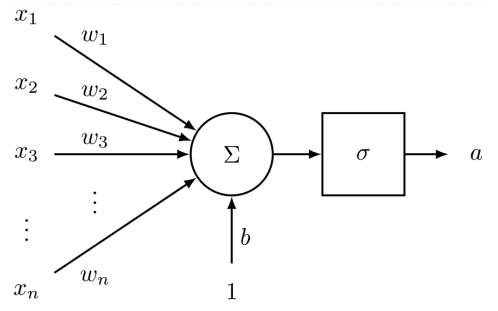
\includegraphics[width=0.45\textwidth]{signalneuralnet.png}}
\subfigure[The structure of neural network]{
\label{Fig.sub.2}
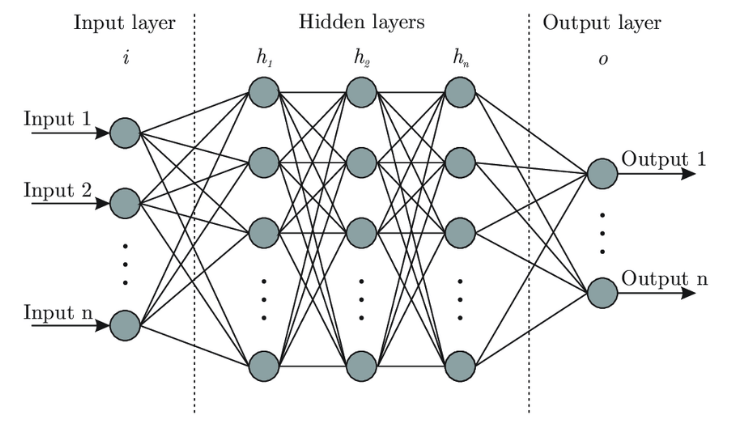
\includegraphics[width=0.45\textwidth]{the-structure-neural-net.png}}
\caption{The structure of neuron and neural network}
\label{Fig.main}
\end{figure}
As shown in Figure 2.1(b), for whole neural network, the first layer is the input layer, the last layer is the output layer, Between the input layer and the output layer is the hidden layer. Depending on the task, the number of neurons in each layer may be different. The number of hidden layers in a neural network can range from zero to more. Empirically, for a wide range of tasks, greater depth does seem to result in better generalisation\cite{goodfellow2016deep}. This suggests that the use of deep architectures does indeed demonstrate a useful priority over the space of functions that the model learns. But in fact, deeper layers may cause over-fitting problems, and at the same time increase the difficulty of training, making it difficult for the model to converge. Therefore, choosing an appropriate number of hidden layers is crucial for building a good neural network
\subsubsection{The Training of Neural Network}
Now that we know the theory of neural networks, only the structure is not enough. We need to let the neural network learn from the samples to complete various tasks. This process is called the training of neural network. When a neural network is being trained, all of its thresholds and weights are initially set to random values. The training data is conveyed to the bottom layer(input layer), and it goes through the following layers, multiplying and adding together in complex ways, until it finally reaches the output layer. The thresholds and weights are continuously adjusted during training process, until training data containing the same labels consistently produce similar outputs\cite{MIT-NN}.
\subsection{Recurrent Neural Network}
\subsubsection{The Theory of Recurrent Neural Network}
Recurrent neural network (RNN) is a kind of artificial neural networks; the difference between it and ordinary neural network is that the connections between nodes in RNN are a directed graph along a temporal sequence. This enables it to show temporal dynamic behavior.RNNs derived from feedforward neural networks can use their internal state (memory) to process input sequences of variable lengths.\cite{dupond2019thorough}. This special structure makes RNN very advantageous when dealing with unsegmented, connected handwriting recognition\cite{fernandez2009novel} or speech recognition.\cite{sak2014long} \cite{li2015constructing}
\subsubsection{The Structure of Recurrent Neural Network}
The recurrent neural network contain input units (input units), the input sets are marked as $x0, x1,..., xt, xt + 1$, and the output sets of output units (output units) are marked as $y0, y1,..., yt, yt + 1$. The recurrent neural network still contain hidden units (hidden units), and we label their output sets as $s0, s1,...,st,st+1$, these hidden units complete most of the main work. You will find in the figure2.2: there is a one-way flow of information from the input unit to the hidden unit, and at the same time another one-way flow of information from the hidden unit to the output unit. In some cases, the recurrent neural network will break the limitation of the interval and guide information from the output unit to the hidden unit. These are called "back projections", and the input of the hidden layer also includes the state of the previous hidden layer. The routines can be self-connected or interconnected.
\begin{figure}[H]
\centering  %图片全局居中
\subfigure[The structure of recurrent neural network]{
\label{Fig.sub.1}
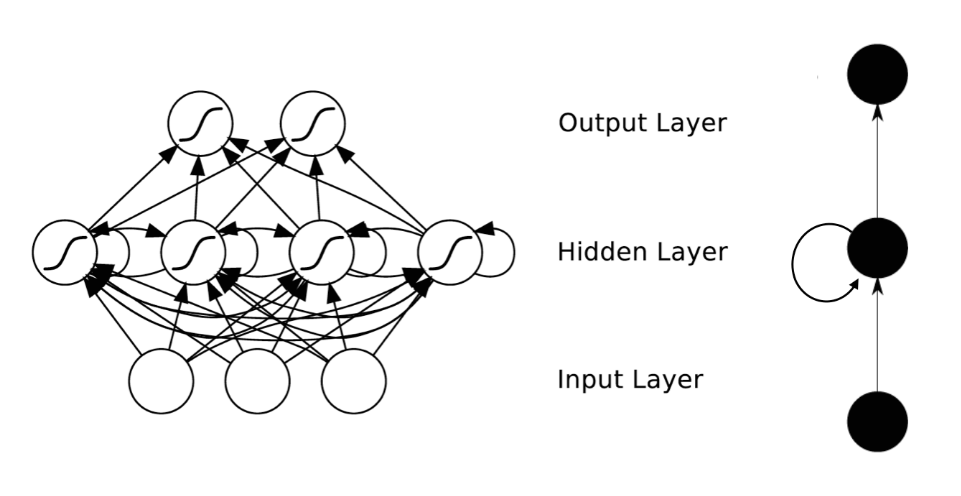
\includegraphics[width=0.45\textwidth]{RNN-structure.png}}
\subfigure[The unfold structure of recurrent neural network]{
\label{Fig.sub.2}
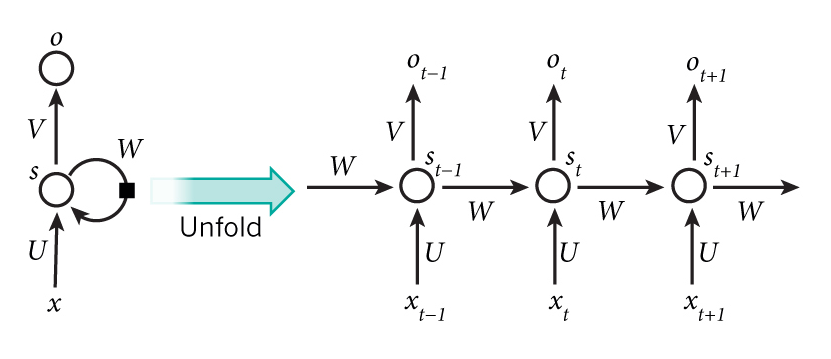
\includegraphics[width=0.45\textwidth]{RNN-structure-unfold.png}}
\caption{The unfold structure of recurrent neural network}
\label{The structure of recurrent neural network}
\end{figure}
\subsection{Long Short-term Memory}
\subsubsection{The Theory of Long Short-term Memory}
Long Short-Term Memory (LSTM) is an artificial neural recurrent network (RNN) architecture that is used in deep learning. \cite{hochreiter9ja1} The difference between LSTM and standard neural networks is that the former has feedback connections. This difference makes lstm can not only process single data points (such as images), but also entire sequences of data (such as speech or video). For example, LSTM is applicable to tasks such as speech recognition, unsegmented, connected handwriting recognition and anomaly detection in network traffic or IDSs (intrusion detection systems).\cite{graves2008novel}
\subsubsection{The Structure of Long Short-term Memory}
As shown in Figure 2.3, in the network structure diagram, each line transmits a vector, which is output from one node and then inputs to another node. The pink circle represents point-by-point operations, such as vector addition; the yellow rectangle represents a neural network layer (that is, a lot of neural nodes); the merged line represents the combination of the vectors carried on the two lines (for example, one vector is $h_{t-1}$, another is $x_{t}$, then the combined output is $[h_{t-1}, x_{t}] $). 

The separated line means that the vector passed on the line is copied and passed to two places. The most critical part of LSTM is the state of the cell (the entire green box is a cell) and the horizontal line on the structure diagram. The transmission of the cell state is like a conveyor belt. The vector passes through the entire cell with only a few linear operations. This structure can easily realize that information can pass through the entire cell without changing it.

If there is only the horizontal line above, there is no way to add or delete information. Lstm is implemented through a structure called gates. The gate can selectively let information through, mainly through a sigmoid neural layer and a point-by-point multiplication operation. Each element of the output of the sigmoid layer (which is a vector) is a real number between 0 and 1, which represents the weight (or proportion) that allows the corresponding information to pass. For example, 0 means "don't let any information pass", and 1 means "let all information pass". Each LSTM has three such gate structures to implement protection and control information\cite{LSTM-github}.
\begin{figure}[H]
\centering  %图片全局居中
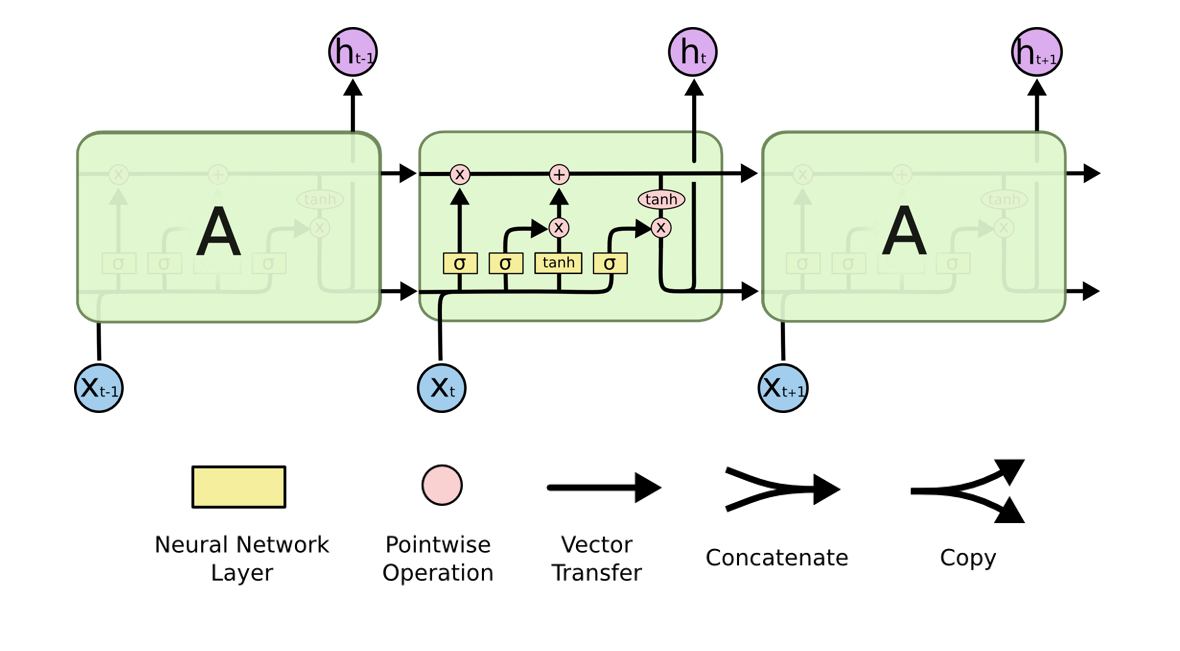
\includegraphics[width=0.7\textwidth]{LSTM.png}
\caption{The structure of long short-term memory}
\end{figure}
\subsubsection{Forget Gate Layer}
As shown in figure 2.4, the first is that LSTM decides to let that information continue to pass through this cell, which is achieved through a sigmoid neural layer called "forget gate layer". Its input is $h_{t-1}$ and $x_{t}$, and the output is a vector with values between 0 and 1 (the length of the vector is the same as the state of the cell $C_{t-1}$), which means that the $C_{t-1}$ is the proportion of each part of the information passed. 0 means "don't let any information pass", 1 means "let all information pass". Going back to the language model mentioned above, the LSTM model has to predict the next word based on all the above information. In this case, the state of each cell should contain the gender information (reserved information) of the current subject so that the LSTM model can use pronouns correctly. But when the LSTM model starts to describe a new subject, the model should forget the gender of the subject (forget the information)\cite{LSTM-github}.
\begin{figure}[H]
\centering  %图片全局居中
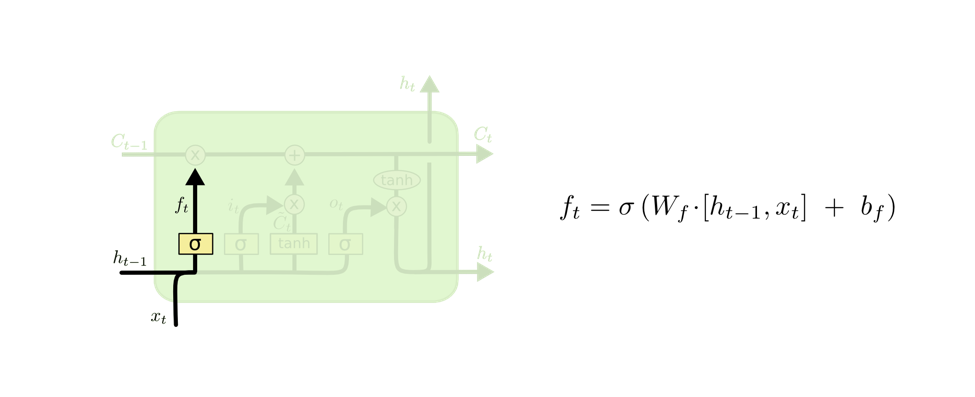
\includegraphics[width=0.7\textwidth]{forget-gate.png}
\caption{The structure of forget gate layer}
\end{figure}
\subsubsection{Input Gate Layer}
The next step is to decide how much new information to add to the cell state. As shown in figure 2.5, this requires two steps: First, a sigmoid layer called "input gate layer" determines which information needs to be updated; a tanh layer generates a vector, $\tilde{C_{t}}$,which is the alternative content for updating. In the next step, the two parts will be combined to update the state of the cell.
\begin{figure}[H]
\centering  %图片全局居中
\subfigure[Input gate layer status 1]{
\label{Fig.sub.1}
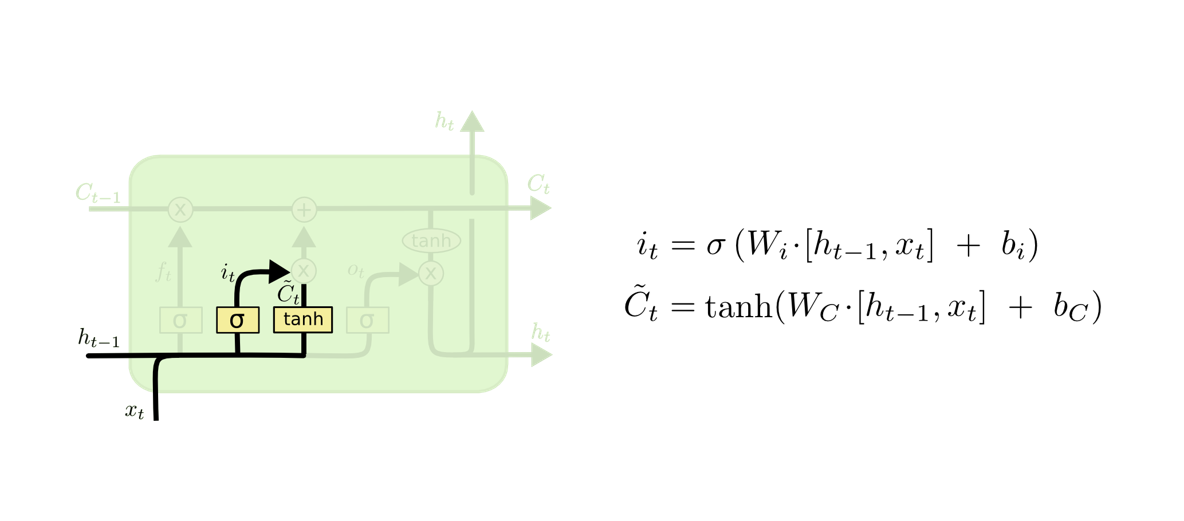
\includegraphics[width=0.45\textwidth]{input-gate.png}}
\subfigure[Input gate layer status 2]{
\label{Fig.sub.2}
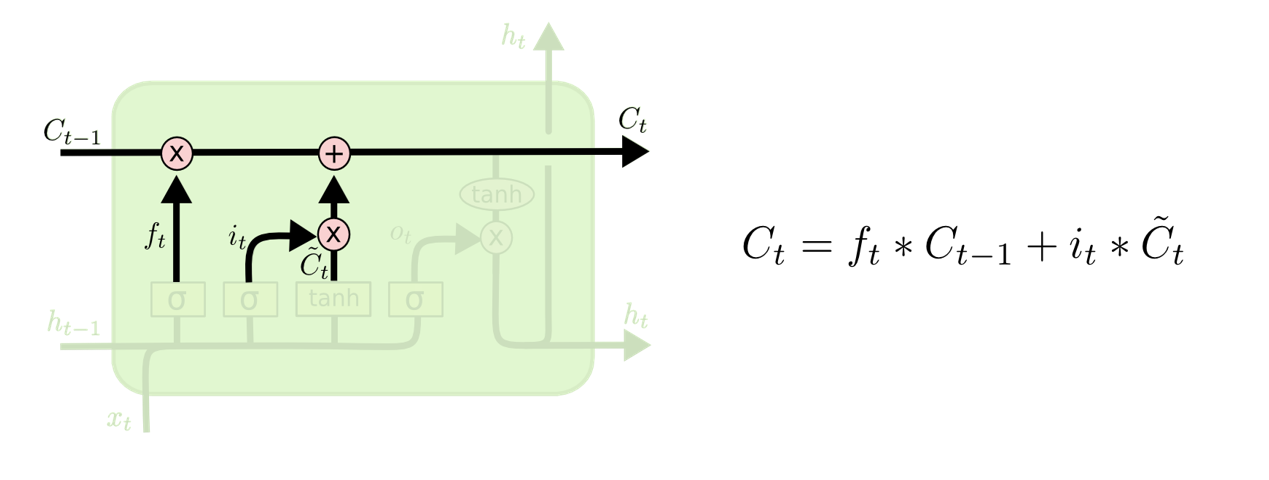
\includegraphics[width=0.45\textwidth]{input-gate2.png}}
\caption{The structure of input gate layer}
\label{The structure of input gate layer}
\end{figure}
In the previous language model example, the LSTM model wants to add new subject gender information to the cell state to replace the old state information. With the above structure, the model can update the cell state, that is, update $ C_{t-1} $ to $C_{t} $. As shown in figure 2.5, first, the model multiplies the old state $C_{t-1}$ with $f_{t}$, this step can let model forget some irrelevant information. The result of previous step will be added with  $i_{t} * \tilde{C_{t}}$. The final result is the new content we want to add \cite{LSTM-github}.
\subsubsection{Output Gate Layer}
The lstm model needs to decide what value to output. This output depends on the state $C_t$ of the cell, but not only depends on $C_t$, it needs to go through a filtering process. As shown in Figure 2.6, first of all, a sigmoid layer will be used to calculate the decision, but need to go through a filtering process. In this filtering process, the LSTM model uses a sigmoid layer (calculated) to determine which part of the information in $C_{t}$ will be output. After that, a tanh layer (return the values between -1 and 1) will be used to calculate a new value base of $C_{t}$. And then, the output of the tanh layer will be multiplied with the weight calculated by the sigmoid layer, so that the final output result is obtained \cite{LSTM-github}.
\begin{figure}[H]
\centering  %图片全局居中
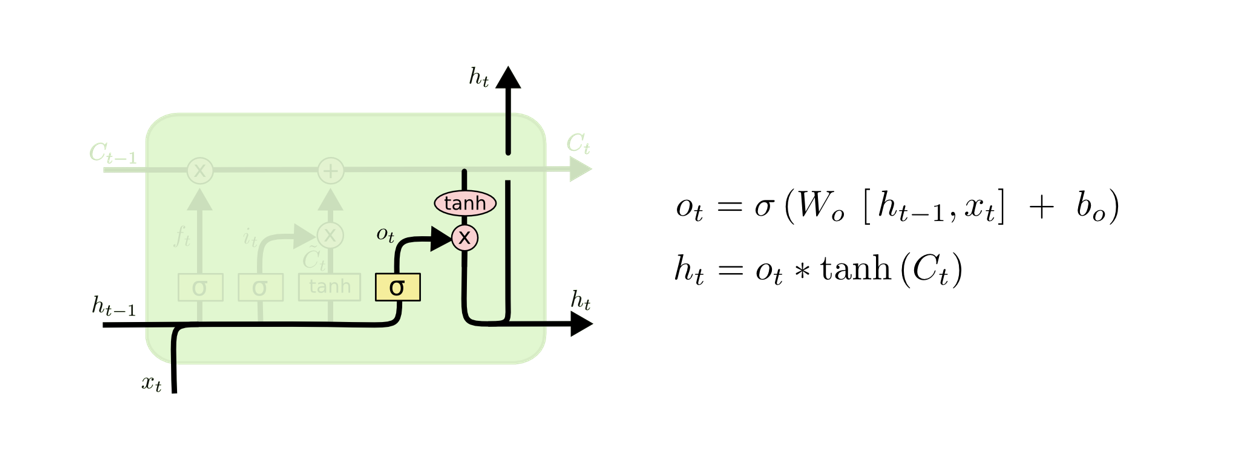
\includegraphics[width=0.7\textwidth]{output-gate.png}
\caption{The structure of output gate layer}
\end{figure}
\section{Information Extraction} 
\qquad Since the content of natural language information on the Internet is mostly repetitive, and the information we focus on is limited, how to extract the content we are interested in from a large amount of text information and convert it into a structured form is our main research objective. Jianshu Weng et al.\cite{d2015real} pointed out that twitter, as a data source of social media, has some common problems with its data, for some real accidents, there are usually a lot of related tweets on Twitter that are meaningless nonsense.
\subsection{The Theory of Information Extraction} 
To solve this problem, we need to implement information extraction (IE) on natural language data. Information extraction (IE) is the task of extracting structured information automatically from unstructured and/or semi-structured machine-readable documents and from other electronically recorded sources. In most cases, information extraction involves processing natural language text with natural language processing techniques. The ultimate objective of information extraction is to facilitate the computation of previously unstructured data. A specific purpose of information extraction is to allow logical reasoning to draw inferences on the basis of the input data 's logical content. Structured data is semantically well-defined data in a chosen target domain, interpreted with respect to category and context\cite{IE-github}.

Charu Virmani et al.\cite{virmani2017extracting} analyzed and summarized the current mainstream information extraction algorithms and analysis methods, including Automatic Summarization, Chunking, Parts-of-Speech Tagging, Named Entity Recognition, etc. Claire Cardie \cite{cardie1997empirical} introduced the architecture of the information extraction system,the first stage is tokenization and tagging, and then sentence analysis, the third stage is extraction, the last stage is merging and template generation. This entire architecture is clear and has a strong guiding role in the development of this project
\subsection{Natural Language Data Preprocessing for Information Extraction}
Natural language data from the network cannot be directly used for information extraction. These natural language data need to be preprocessed first. The main natural language data preprocessing steps include Tokenisation, Part-of-speech Tagging, Named Entity Recognition, etc. These steps will be introduced in the next section.
\subsubsection{Tokenisation}
\qquad Breaking the raw text into small chunks is the main content of tokenization. Tokenization splits the raw text into words, sentences defined as tokens. These tokens can help to understand the context or to create an NLP model. The tokenization is helpful in interpreting the meaning of the natural language data by analyzing the sequence of the words. For example, the text "It is a chair" can be tokenized into "It", "is", "a", "chair". As the most basic step in natural language processing, there are different methods and libraries available to perform tokenization. NLTK \cite{NLTK-doc}, Gensim \cite{gensim-doc}, Keras \cite{Keras-doc} are the libraries which can be used to accomplish the mission. Tokenisation can be achieved either to separate words or phrases. 
\subsubsection{Part-of-speech Tagging}
Tagging is a sort of classification that can be described as automatic description assignment to the tokens. The descriptor is called tag, which can represent one of the part-of-speech, semantic information and so on. In simple words, POS tagging is a task of labelling each word in a sentence with its appropriate part of speech. Part-of-speech tagging is more complicated than just providing a list of words and their parts of speech, since certain words can represent more than one part of speech at different times, and there are some parts of speech are complex or unspoken. This is not unusual — there are a large percentage of word-forms are ambiguous in natural languages (as opposed to many artificial languages). For instance, even "dogs", which is generally considered as just a plural noun, can also be a verb: The sailor dogs the hatch. For that sentence, a correct tagging should reflect that "dogs" is here used as a verb, not as the more common plural noun \cite{POS-wiki}.
\section{Named Entity Recognition}
\qquad Named-entity recognition (NER) (also known as entity identification, entity chunking and entity extraction), refers to the recognition of entities with specific meanings in the text, including names of people, places, organizations, proper nouns, etc. Named entity recognition is an important basic tool in application fields such as information extraction, question answering systems, syntax analysis, machine translation, Semantic Web-oriented metadata annotation, and it occupies an important position in the process of natural language processing technology becoming practical. Generally speaking, the task of named entity recognition is to identify three categories (entity category, time category and number category) and seven categories (person name, organization name, place name, time, date, currency and percentage) in the text to be processed.
\cite{NER-wiki}

\subsection{Challenges in Named Entity Recognition}
Named entity recognition consists of the following two sub-problems: (1)recognition of named entity boundaries; (2) recognition of named entity categories(classes). These problems are usually (but not necessarily) addressed concurrently. As with most language handling issues, there are ambiguities in the language that adds to the challenge of the task. Heavily lexicalized and domain-dependent nature is key challenges to named entity recognition. A large part of a language are names which are constantly evolving in different domains. A robust named entity recognition system for any domain needs labeled corpora and lexicons (e.g., names of monuments). It is expensive to create and update such resources for a number of topics, and it also requires linguistics and domain expertise. There are two popular frameworks of named entity recognition, rule-based and statistical NER. They will be introduced in the following sections\cite{zitouni2014natural}.
\subsection{Rule-Based Named Entity Recognition}
Early approaches to the recognition of named entities were mainly based on rules. The majority of systems based on rule used three main components : a group of named extraction rules, gaseous (a domain specific lexicon) for the various kinds of named entity classes,an extraction engine that applied the rules and the text lexicons.\cite{zitouni2014natural} Rule-based named entity recognition systems are relatively precise but usually have low coverage and work well on narrow domains. Usually their performance depends on the comprehensiveness of the rules and lexicons. Frameworks such as \cite{riloff2004introduction} are still restricted to the seed rules and the lexicon domain. In addition, it is costly to manually integrate deeper information in a rule-based structure beyond surface terms and lexicons. Statistical frameworks, by contrast, are more flexible in incorporating richer linguistic knowledge ( e.g., syntax), resulting in more robust systems.
\subsection{Statistical Named Entity Recognition}
Named entity recognition work has concentrated on data-driven and statistical methods due to an growing adoption of NLP statistical methods as well as expanding available data resources. By using statistical methods, the human effort for the tedious construction of rule sets and gazeteers has been reduced. Shortly after their development, the performance of statistical and hybrid systems like \cite{mikheev1999named}\cite{miller1998bbn} is better than the state-of-the-art rule-based systems. There are two components usually used in statistical named entity recognition: (1) labeled training data: text corpora where named entities are annotated  (2) a statistical model: a probabilistic representation of the training data. A statistic model consists of parameters that map a  language event to a probability.
Named entity recognition can be modelled as a classification task for each individual token as a supervised learning problem. Such an approach, however, fails to consider the interdependence between various tokens. In contrast, named entity recognition is usually seen as a structured learning problem for a sequence of variables. This is the view of the sequence labelling where the learner predicts the labels for the whole sequence of tokens (usually as entence). The modelling of the dependency is allowed to exist between tokens under this method\cite{zitouni2014natural}.

\section{Accident Detection in Social Media}
\qquad So far, natural language processing technology has been very widely used on social media, and there has been a lot of research focused on accident detection on social media and news websites. Hamed Abdelhaq et al. \cite{abdelhaq2013eventweet} proposed a system that not only detects accidents in real-time Twitter data streams, but also tracks the evolution of accidents. Fabian Abel et al. \cite{abel2012twitcident} presented an framework, Twitcident, which can search, filter, analysis information about events or crises in real world. When incident occurs, this framework can track and filter data from Twitter. Michael Hund et al.%\cite{krstajic2012getting} 
developed a methodology for real-time event detection by recognising keywords whose frequency is dramatically higher than expected. Axel Schul et al.\cite{schulz2013see} uses semantic web technologies combined with machine learning to identify microblogs related to accidents with an accuracy rate of up to 89\%. Eleonora D'Andrea \cite{d2015real} presented an analysis of the Twitter stream in real-time traffic event monitoring network. Their programme used SVM to identify tweets as traffic events or not, and achieved an accuracy of 95.75 per cent. 


% Local Variables: 
% mode: latex
% TeX-master: "report"
% End: 
